\graphicspath{ {./resources/nav/} }
\documentclass[../templateLTHtwocol.tex]{subfiles}
\begin{document}

The objective for the RL agent is to hover at $S_t = [0, 0, 1]$ starting from the origin $S_0 = [0, 0, 0]$. Throughout the training iterations, the starting point remains fixed. Once trained, we evaluate the RL policy in a similar setting to the training task, i.e. starting at the origin, but also test the ability to generalize by changing the starting point to an arbitrary location which was never explored by the agent during training, we also subject agent to external disturbances (wind) while evaluating the model in real-world.

The results are presented and compared for the three approaches described before i. Pure RL. ii. RL with open loop control. iii. RL with closed loop control. Table \ref{rl_ts:table} summarizes the results. The pure RL approach (directly controlling the motor RPMs) was not found to converge even after training for 10 million steps. The RL with the open loop control approach managed to converge after ~10 hrs of training, while the custom implementation of RL and a PID loop managed to converge in significantly less training time and achieves a better-expected reward (reward per step in the episode). Figure \ref{nav_hov_oc:fig} compare the results of approaches (ii) and (iii). We see that the agent in approach (iii) learns significantly faster and manages to attain a higher reward early in the training phase and also attains a higher expected reward at the end of training. This is due to the fact that the agent has robust low-level control to execute the necessary motion primitives (using a closed loop PID controller) and does not have to learn them from scratch, unlike approach (ii). It is also worth noting that the magnitude of expected reward in (iii) is quite high compared to (ii), a negative reward of -6 vs -3 (per step), this is again due to the fact that we leverage robust low-level control, because of which the agent can execute actions concretely and explore more of the environment.
The actor reward after convergence is close to about 1, which is expected, as the shortest distance between $S_0 = [0, 0, 0], S_t = [0, 0, 1]$ is 1 (Euclidean distance).

Approach (iii) was simulated after training converged. Figure \ref{rl_c_3d-plot000:fig} is the same as the training task, with the starting point being the origin. In figure \ref{rl_c_3d-plot333:fig}, the starting point was chosen arbitrarily, $S_0=[3, 3, 3]$, which was never explored by the agent during the training phase, yet the policy generalizes well, but the subtle thing to note is that the trajectory is not entirely optimal (the shortest path between two points is a straight line), instead the agent first navigates to a location close to the destination and then pursues a familiar trajectory encountered during training.

The model was also tested to control the real hardware and the results were similar. While testing on the real hardware, external disturbances were applied in attempts to drift the CF2.X from the hovering point, and the model could stabilize fairly stabilize and return to the hovering point.

\begin{table}[H]
\caption{Training Summary}
\label{rl_ts:table}
\centering
\begin{adjustbox}{max width=0.45\textwidth}
\begin{tabular}{|l|c|c|c|}
\hline
\multicolumn{1}{|c|}{\textbf{Metrics}} & \multicolumn{3}{c|}{\textbf{Approach}}                                                                               \\ \hline
\multicolumn{1}{|c|}{\textbf{}}        & \multicolumn{1}{c|}{\textbf{Pure RL}}         & \multicolumn{1}{c|}{\textbf{RL + Open loop}} & \textbf{RL + Closed loop} \\ \hline
\multicolumn{1}{|l|}{\textbf{Description}}          & \multicolumn{1}{c|}{\begin{tabular}[c]{@{}c@{}}No controller needed, the RL agent\\  learns to execute the \\ low-level actions on its own.\end{tabular}} & \multicolumn{1}{c|}{\begin{tabular}[c]{@{}c@{}}The open-loop makes the RL\\  task easier, but the execution \\ of actions is not consistent.\end{tabular}} & \multicolumn{1}{c|}{\begin{tabular}[c]{@{}c@{}}Abstracts all of the low-level control\\  from RL and ensures consistency\\  in action execution\end{tabular}} \\ \hline
Number of Timesteps                    & \multicolumn{1}{c|}{\textgreater 10 Million} & \multicolumn{1}{c|}{$\sim$1 Million}         & $\sim$100 K            \\ \hline
Training Time $\dag$                   & \multicolumn{1}{c|}{\textgreater 13 hrs}     & \multicolumn{1}{c|}{$\sim$10 hrs}            & $\sim$1.5 hrs          \\ \hline
Expected Reward                        & \multicolumn{1}{c|}{-}                       & \multicolumn{1}{c|}{-0.4}                    & -0.1                   \\ \hline
Convergence                            & \multicolumn{1}{c|}{No}                      & \multicolumn{1}{c|}{Yes}                     & Yes                    \\ \hline
\multicolumn{4}{l}{\footnotesize $\dag$ all training durations are reported on the same hardware}\\
\end{tabular}
\end{adjustbox}
\end{table}

\begin{figure*}[h]
	\centering
	\caption{RL Training Performance: Comparison of RL + Open Loop Control and RL + Closed Loop Control}
	{Figures plotting the RL results for the task of hovering using open loop control to execute the actions. The X-axis represents the relative timesteps. The Y-axis represents the magnitude. Total number of timesteps for RL + open loop system is 1\,000\,000 (1 M), and 100\,000 (100 K) for the RL + closed loop system. The performance metric used here is the expected reward per step (higher the better)}
	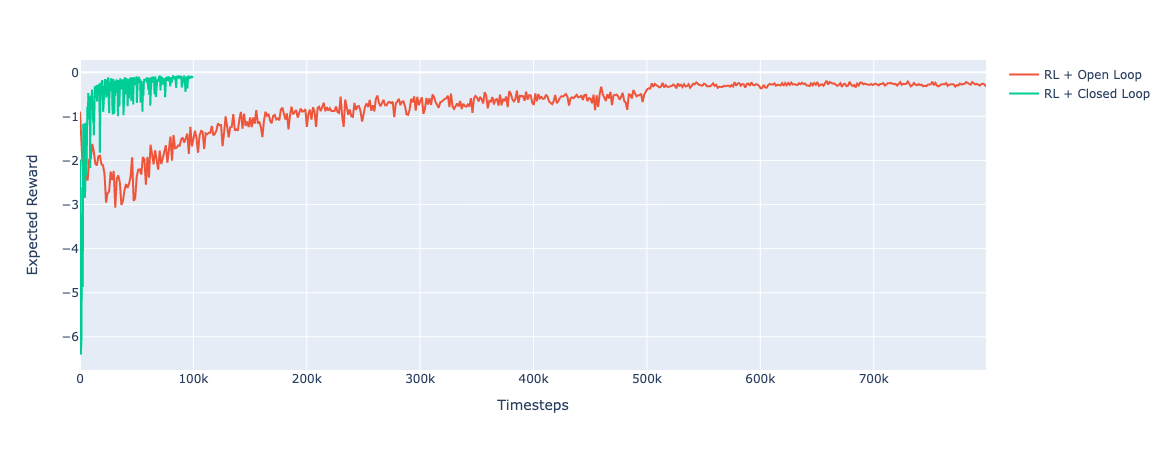
\includegraphics[scale=0.4]{rl_c_o_rewards.png}
	\label{nav_hov_oc:fig}
\end{figure*}

\begin{figure}[H]
	\centering
	\caption{RL Policy Test}
	{The plots trace the movements of the agent in the environment. Red indicates the starting point and green is the destination.}

	\begin{subfigure}[b]{0.25\textwidth}
		\caption{Case 1: Starting at origin (same as training task)}
		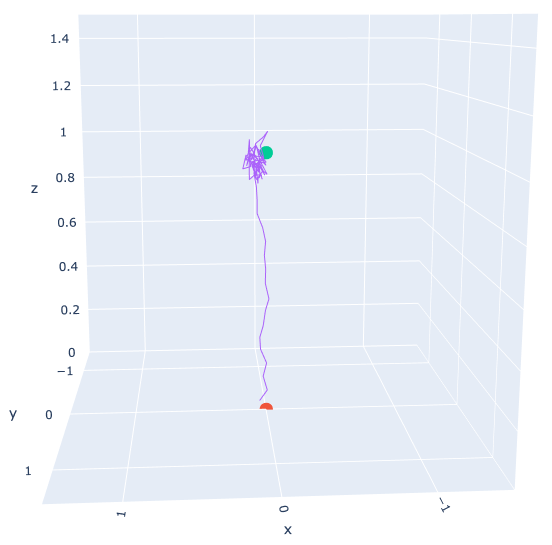
\includegraphics[width=\textwidth]{rl_c_3d-plot000.png}
		\label{rl_c_3d-plot000:fig}
	\end{subfigure}
	\hfill
	\begin{subfigure}[b]{0.25\textwidth}
		\caption{Case 2: Starting at an arbitrary location (trajectory not explored during training)}
		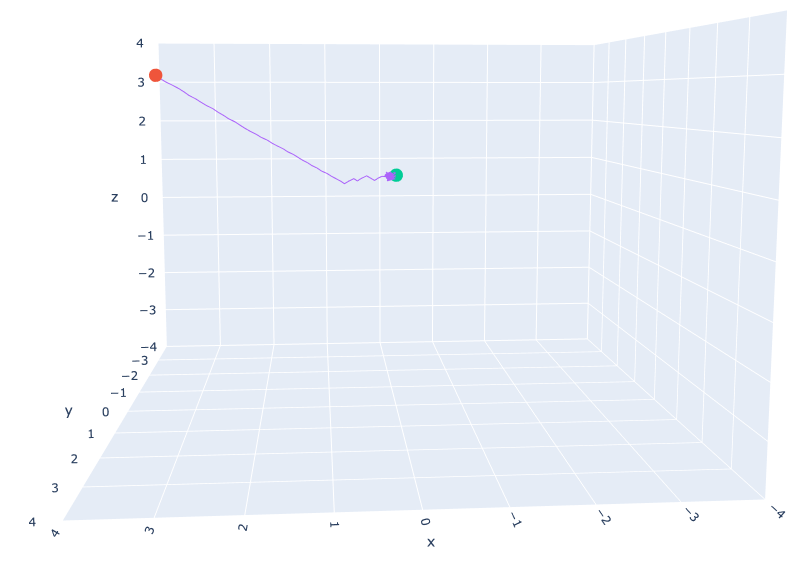
\includegraphics[width=\textwidth]{rl_c_3d-plot333}
		\label{rl_c_3d-plot333:fig}
	\end{subfigure}
\end{figure}

\end{document}
